\documentclass[12pt,letterpaper]{article}
\usepackage[utf8]{inputenc}
\usepackage[english]{babel}
\usepackage{listings}
\usepackage{xcolor}
\usepackage{graphicx}

\title{\textbf{Department of Computer Science and Engineering}}
\author{\textbf{S.G.Shivanirudh , 185001146, Semester V }}

\date{14 October 2020}

\begin{document}
\maketitle
\hrule
\section*{\center{UCS1511 - Networks Laboratory}}
\hrule 
\bigskip\bigskip

%Assignment name
\subsection*{\center{\textbf{Exercise 8: Performance Evaluation of TCP and UDP}}}

%Objective
\subsection*{\flushleft{Objective:}}
\begin{flushleft}
Write ns2 program to do Performance Evaluation of \textbf{TCP and UDP sharing a bottleneck link.}
\end{flushleft}

%Code
\subsection*{\flushleft{Simulation Code:}}
\begin{flushleft}
\lstinputlisting[language = TCL, firstline = 3, lastline = 101]{tcpudp.tcl}

\newpage
\subsection*{\flushleft{Inferences:}}
\begin{itemize}
	\item The following specifications defined the connections in the TCL script.
	\begin{itemize}
	\renewcommand\labelitemi{-}
		\item 0 $\longrightarrow$ 2 has a duplex link with a bandwidth of 2Mb and 10ms transmission delay.
		\item 1 $\longrightarrow$ 2 has a duplex link with a bandwidth of 2Mb and 10ms transmission delay.
		\item 2 $\longrightarrow$ 3 has a simplex link with a bandwidth of 0.3Mb and 100ms transmission delay.
		\item 3 $\longrightarrow$ 2 has a simplex link with a bandwidth of 0.3Mb and 100ms transmission delay.
		\item 3 $\longrightarrow$ 3 has a duplex link with a bandwidth of 0.5Mb and 40ms transmission delay.
		\item 3 $\longrightarrow$ 5 has a duplex link with a bandwidth of 0.5Mb and 40ms transmission delay.
	\end{itemize}
	\item A FTP and CBR applications used the established TCP over 1 and 4, and UDP over 0 and 5 respectively.
	\item Starting from a lossless packet transfer, a build up of packets in the queue of the bottleneck link 2 $\longrightarrow$ 3 occured.
	\item Due to being overloaded, the \textbf{DropTail} protocol started taking effect around 3.36 seconds, when the first packet is dropped from 2, and continued till approximately 3.84 seconds. This process completely stopped once the load eased up from the termination of the FTP application at 4.7 seconds.
	\item Any bottleneck in a network affect the efficiency of the entire network, leading to loss of data.
	\item Solutions to this problem include:
	\begin{itemize}
	\renewcommand\labelitemi{-}
		\item Adaptive transmission rates.
		\item Adjusting queue size.
		\item Increase bandwidth and/or reduce transmission delay of bottleneck link.
	\end{itemize}
\end{itemize}	

%Output
\subsection*{\flushleft{Output:}}
\begin{figure}[h]
    \centering
    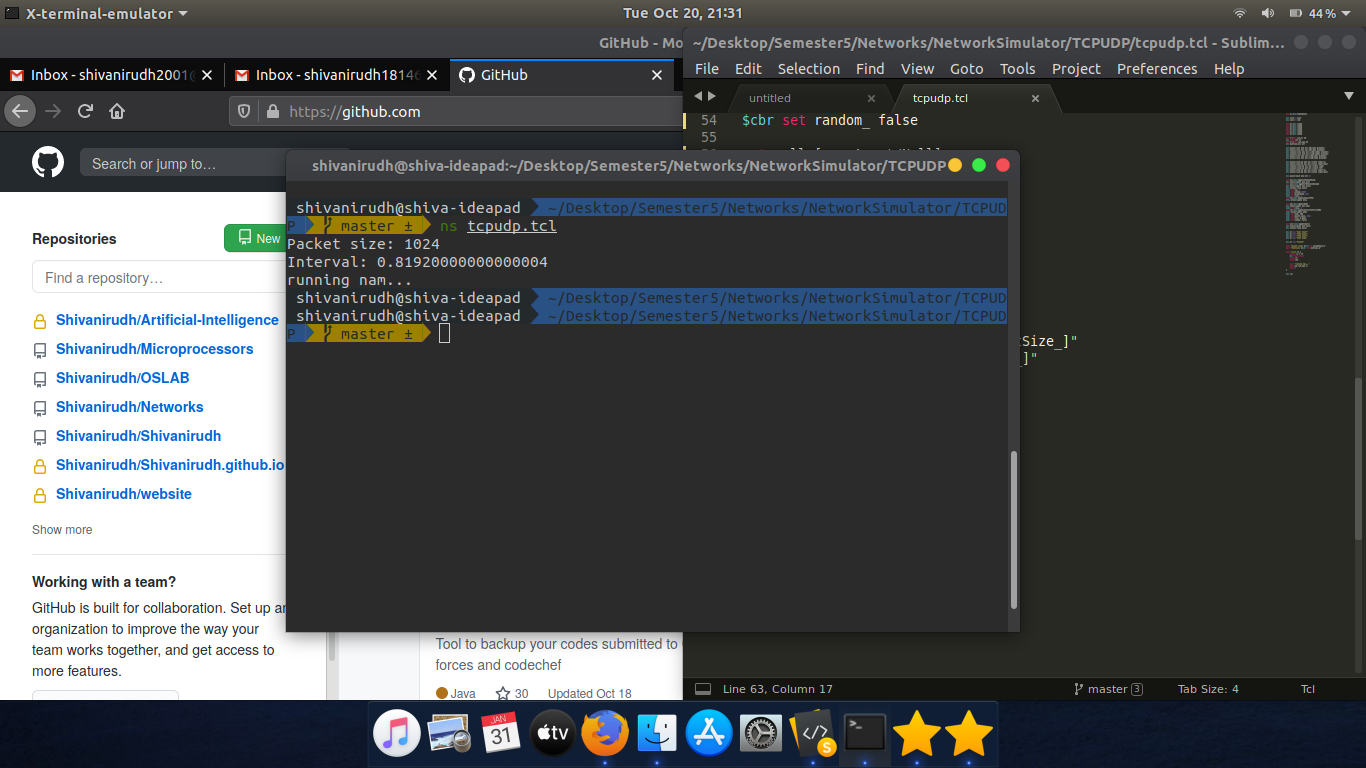
\includegraphics[trim = 100mm 50mm 125mm 70mm, clip, width = \textwidth]{Pics/TerminalRun.png}
    \caption{ \textbf{CBR Packet Size:} 1024, \textbf{CBR Interval}: 0.8192s}
\end{figure}
\begin{figure}[t]
    \centering
    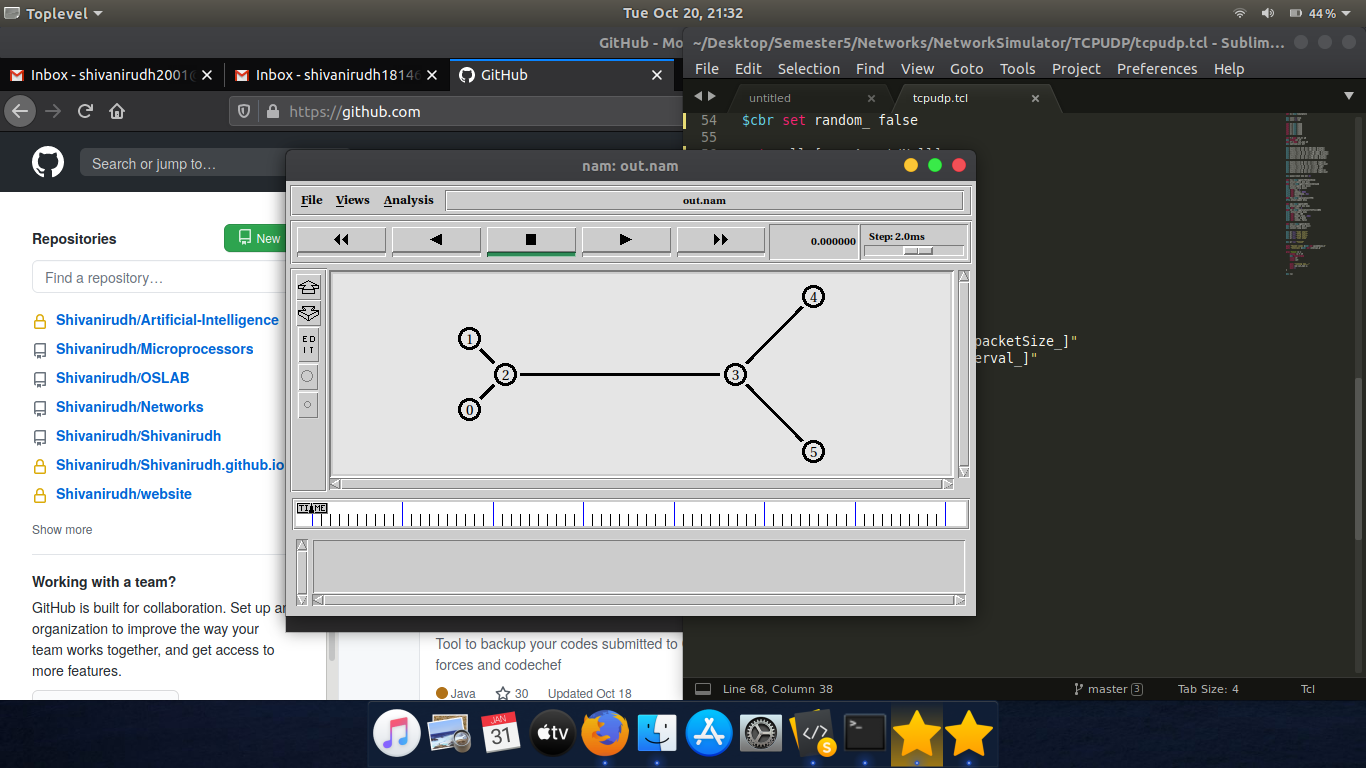
\includegraphics[trim = 100mm 50mm 135mm 70mm, clip, width = \textwidth]{Pics/NodeGraph.png}
    \caption{\textbf{Node Structure}}

    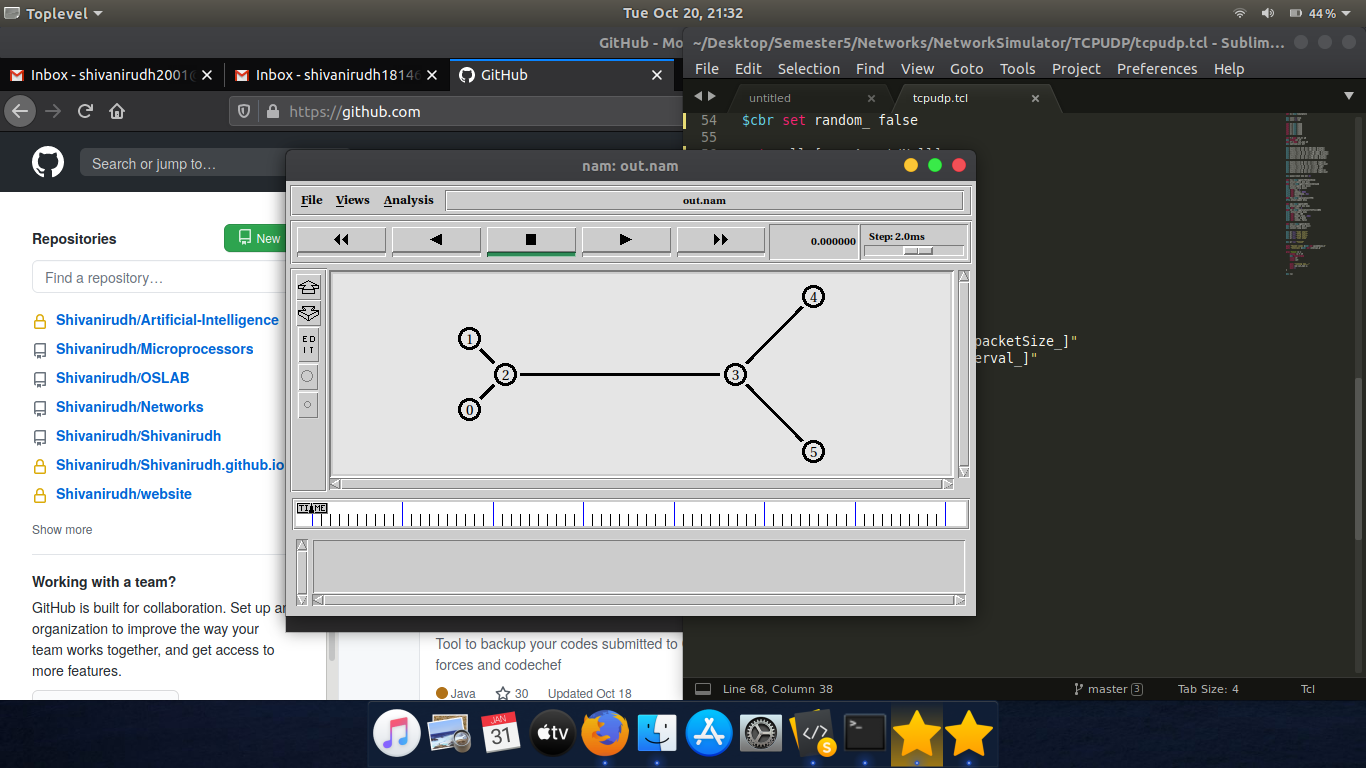
\includegraphics[trim = 100mm 50mm 135mm 70mm, clip, width = \textwidth]{Pics/NodeGraph.png}
    \caption{\textbf{N1 to N5 UDP connection CBR}}
\end{figure}
\begin{figure}[t]
	\centering
    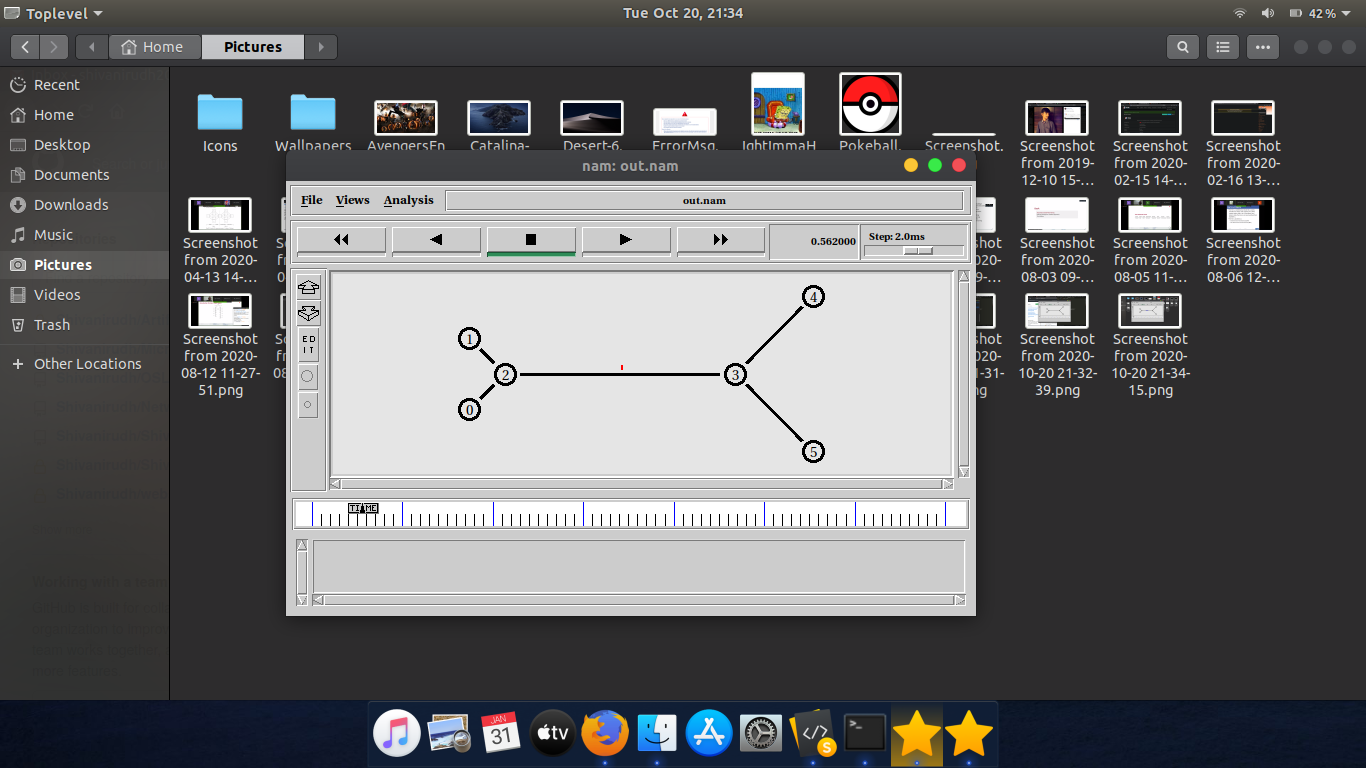
\includegraphics[trim = 100mm 50mm 135mm 70mm, clip, width = \textwidth]{Pics/TCPAck.png}
    \caption{\textbf{N1 to N4 TCP connection acknowledgement}}

    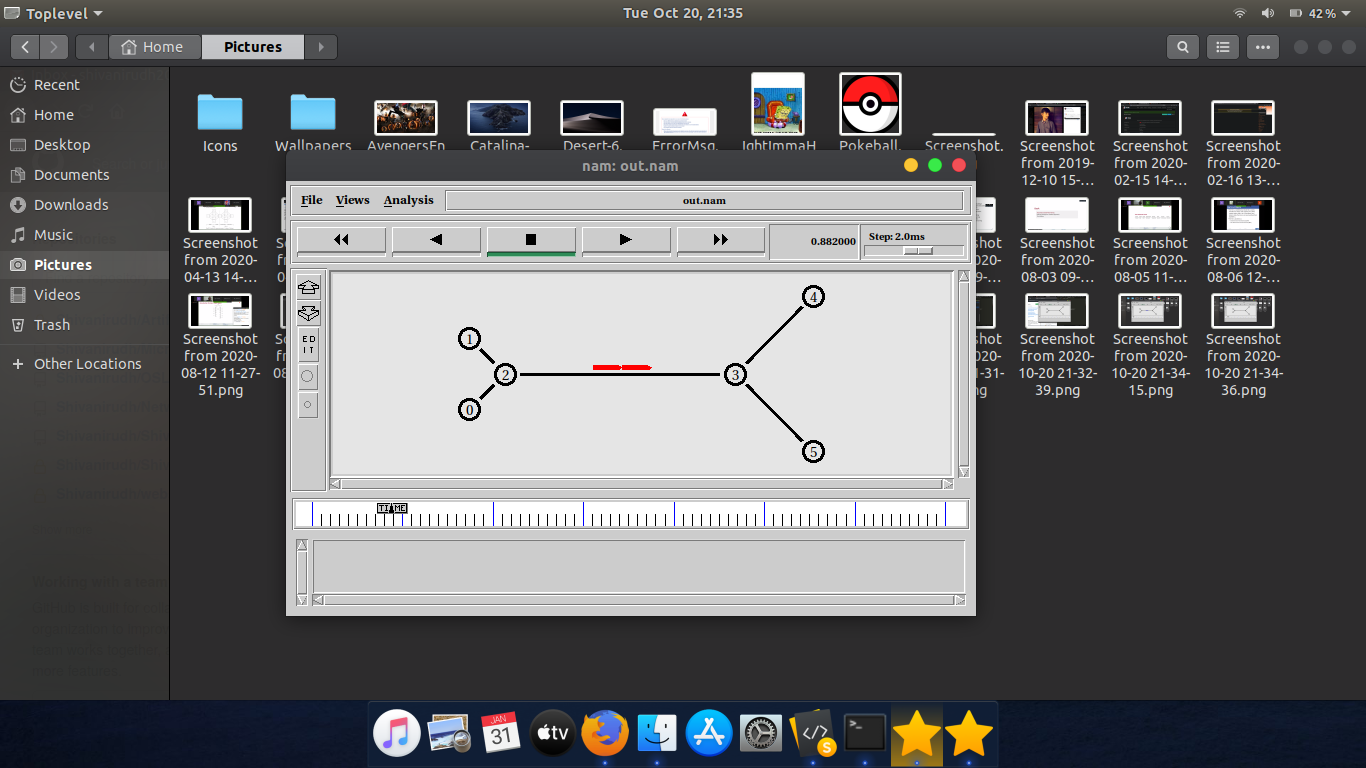
\includegraphics[trim = 100mm 50mm 135mm 70mm, clip, width = \textwidth]{Pics/TCPTrans.png}
    \caption{\textbf{N1 to N4 TCP connection packet transmission}}
\end{figure}
\begin{figure}[t]
	\centering
    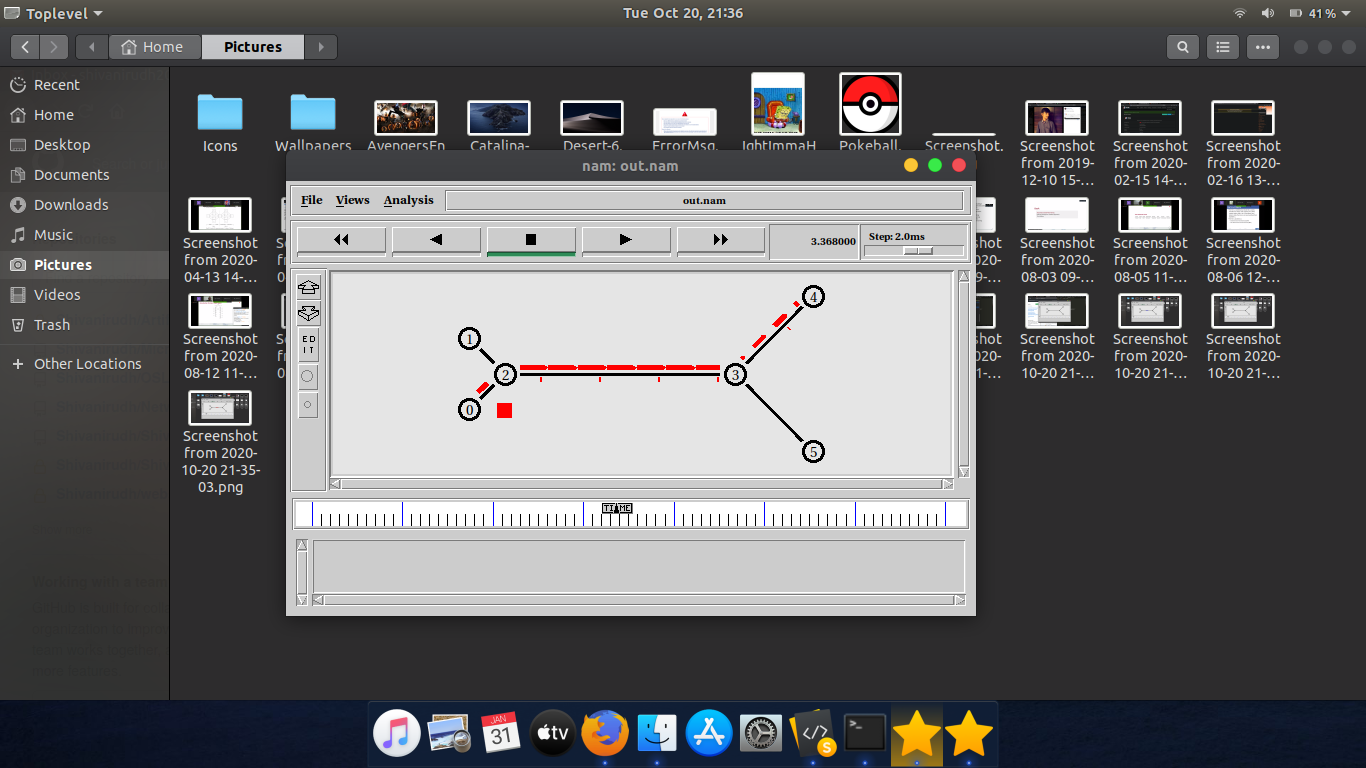
\includegraphics[trim = 100mm 50mm 135mm 70mm, clip, width = \textwidth]{Pics/Firstdrop.png}
    \caption{\textbf{First packet drop}}

    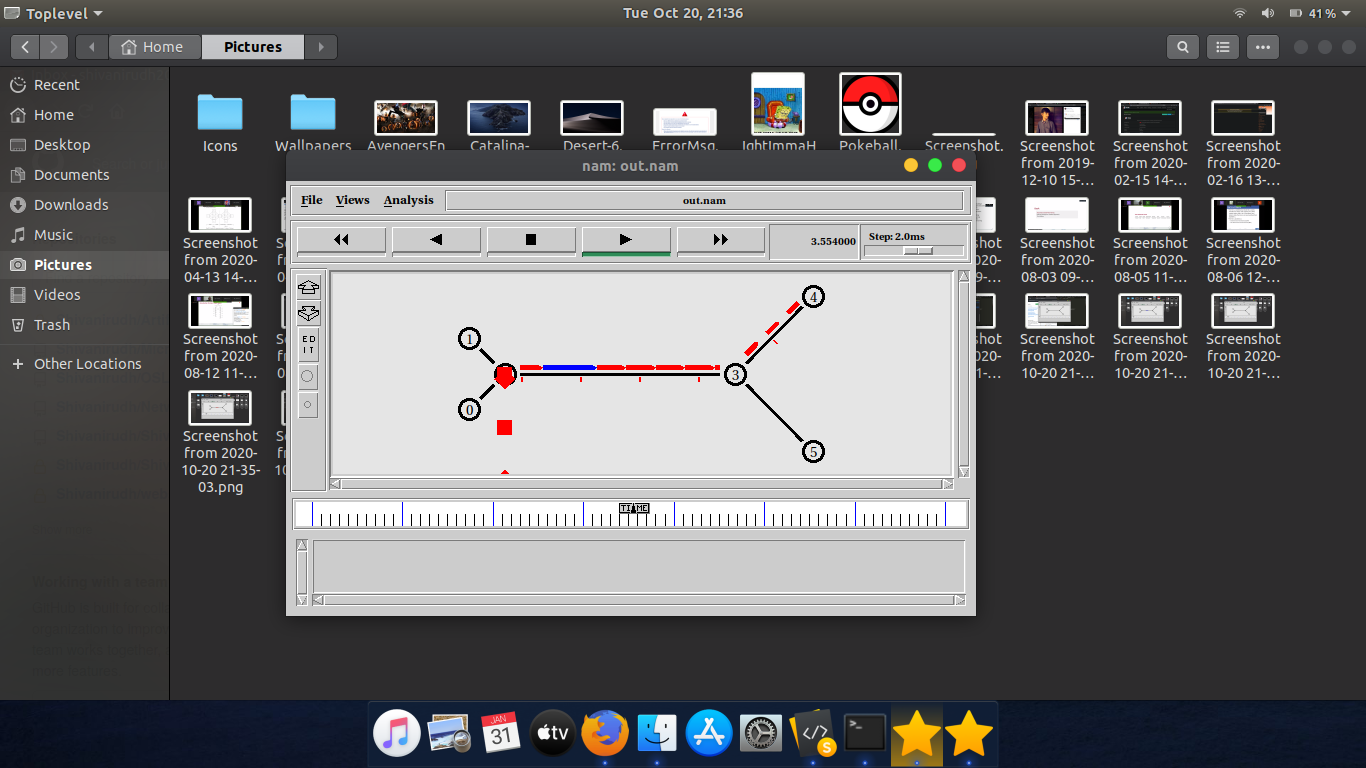
\includegraphics[trim = 100mm 50mm 135mm 70mm, clip, width = \textwidth]{Pics/Packetdrop.png}
    \caption{\textbf{Rest of the packets drop}}
\end{figure}

\end{flushleft}
\end{document}